\documentclass[a4paper]{report}
\usepackage{hyperref}
\usepackage{lastpage}
\usepackage{fancyhdr}
\usepackage{lineno}
\usepackage{listings}
\usepackage{german}
\usepackage[utf8]{inputenc}
\usepackage{amssymb}
\usepackage{graphicx}
%\newcommand{\genasso}[2]{\begin{minipage}{0.7\textwidth}\begin{normalsize}\begin{flushleft}\textbf{{#1}}\end{flushleft}\end{normalsize}\vspace{-1cm}\begin{flushleft}\begin{small}{#2}\end{small}\end{flushleft}\end{minipage}\\\vspace{0.2cm}}
\pagenumbering{arabic}

\pagestyle{fancy} 
\newcommand{\frontmatter}{\clearpage \cfoot{\thepage\ }
\setcounter{page}{1}
\pagenumbering{Roman}}
\newcommand{\mainmatter}{\clearpage \lhead{\myAuth} \rhead{\myDate} \cfoot{} \rfoot{\thepage\ of \pageref{LastPage}}
\setcounter{page}{1}
\pagenumbering{arabic}}
\newcommand{\backmatter}{\clearpage \rfoot{\thepage\ }
\setcounter{page}{1}
\pagenumbering{alph}}


\newcommand{\makemytitlepage}{\begin{titlepage}
    \begin{center}
        \vspace*{0.8cm}
        
        \Huge
        \textbf{\myTitle}
        
        \vspace{1.5cm}
        
        \Large
        \myAuthor

        \vspace{1.8cm}

        %\begin{large}\textbf{Abstract:} \myAbstract \end{large}
        
\includegraphics[width=6cm]{./IM.jpg}  
        
        \vfill
        
        \huge
        \myAsso
        
        \vspace{1.3cm}
        
        \Large

        %\myDate
        \today
        
    \end{center}
\end{titlepage}}
\newcommand{\myAuth}{Team: *Iron Man*\\B. Pohl, K. Trogant, R. Enseleit, D. Hebecker}
\newcommand{\myAuthor}{Birgit Pohl 574353 (MO. 9-11)\\Kevin Trogant 572451 (Mo. 15-17)\\Ronja Enseleit 572404 (Mo. 15-17)\\Dustin Hebecker 571271 (MO. 9-11)}
\newcommand{\myAsso}{Group: *Iron Man*}
\newcommand{\myDate}{\today}

%%%%%%%%%%%%%%%%%%%%%%%%%%%%%%%%
%%Change Title !!!!!!!!!!!!!!!!!
%%%%%%%%%%%%%%%%%%%%%%%%%%%%%%%%
\newcommand{\myTitle}{Exercise Sheet 7}

\begin{document}
\frontmatter
\makemytitlepage
\mainmatter

%%%%%%%%%%%%%%%%%%%%%%%%%%%%%%%%%%%%%%%%%%%%%%%%%%%%%%%%%%
%% Only modify below here  and change myTitle!!!!!!!!!!!!!
%%%%%%%%%%%%%%%%%%%%%%%%%%%%%%%%%%%%%%%%%%%%%%%%%%%%%%%%%%
\section*{Aufgabe 1}
You can find the setup guideline in the README.md.

\newpage
\section*{Aufgabe 2}
For the test-driven-development we chose Cucumber to define a brief functionality without implementing the functionality. It is based on Gherkin and it is so easy to read, that even non-developers can understand what is happening in each scenario and they are able to come up with own suggestions.
Planning with Cucumber makes it easy to identify unforeseen cases. We have managed to simplify the test-cases, which in the end simplified the program itself. But this is not enough, while communicating with the group to implement the program based on Cucumber, we saw that we still defined to much functionality and therefore, we decided to take them out as well.

While implementing the program, we defined the step definitions for the tests. The place where tests pass or fail. While working on the program's implemention until the early morning, one or another mistake sneaked into our program, but our reliable test setup - of course - caught them all, even it's own mistakes. That is how we have managed to correct the isCousinOf and getCousinOf methods, which went true when one asks, if the parent and a his child are cousins. We know that, because we were debugging it on the step definition's side.
Debugging with the scenario.write() methode makes it possible to print statements during the tests. It helped us to make all women females again, when they accidentally were made male by our test.

We manually tested our program as well, and we decided to add more functionality. Our tests clearly separates the methods of the family tree, therefore we didn't encounter new test failures after changing the program.

Cucumber is made for many programming languages. We use Cucumber for Java, which also needs Maven and JUnit in IntelliJ to function. So far, we have not managed to implement a test-coverage due to a bug by Oracle which is introduced in JDK 1.7 and it is still not fixed in JDK 1.8. But the test-coverage for Javascript applications work like a charme.

Cucumber and Gherkin are well known in the industry:

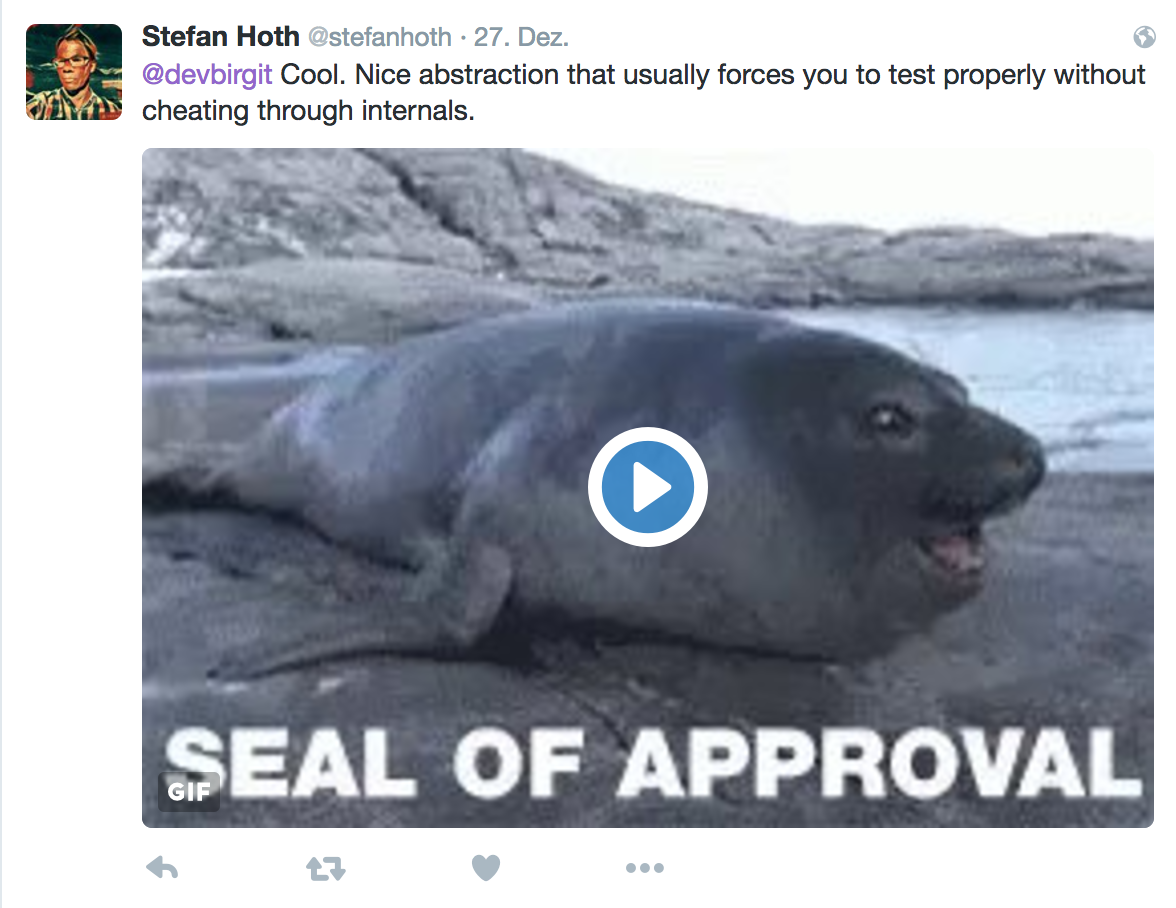
\includegraphics[width=6cm]{./SealOfApproval.png}

Stefan Roth (City kid | Community builder | Amateur Photographer | Mentor | Opinion-haver | Runs @BerlinHacknTell & @GDGBerlin | Enjoys working at @novoda)




%Hello World 
%\begin{lstlisting}
%Put your code here.
%\end{lstlisting}



\end{document}
